\chapter{Resultados \label{chap:Resultados}}
%%%%%%%%%%%%%%%%%%%%%%%%%%%%%%%%%%%%%%%%%%%%%%%%%%%%%%%%%%%%%%%%%%
\noindent Habiendo calculado y aplicado los valores de expectación, $\mu_{g}$ y $\mu_{bkg}$, para corregir la carga sobre los clusters y habiendo introducido el modelo de la colección parcial de carga, que es usado en el ajuste de los espectros, ya se pueden presentar los resultados derivados de estos.

Inicialmente se presentan los resultados obtenidos al aplicar el modelo de ajuste a los datos sin ningún tipo de aplicación de umbral ni de corrección de datos, es decir, se uso un \verb|EPIX|$=0.5$ y se ajustaron los espectros, tanto para el flúor como para el aluminio utilizando el modelo previamente descripto. De esto se obtuvieron los resultados de la figura \ref{fig:OHDU1_EPIX05}, \textit{para el primer cuadrante del sensor}, donde se ve que el factor de Fano es de $F = 0.1322 \pm 0.0022$ y la energía de creación electrón hueco para el aluminio es $\varepsilon_{\eh} = 3.7141 \pm 0.0019$
\begin{figure}[H]
    \centering
        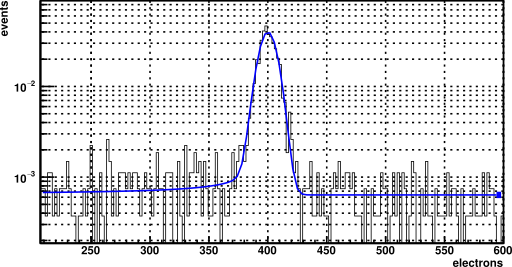
\includegraphics[scale=1]{pngs/OHDU1_EPIX05.png}
    \caption{\footnotesize{asd.}}
    \label{fig:OHDU1_EPIX05}
\end{figure}
En segundo lugar, se aplica el umbral con \verb|EPIX|$=1.5$, con lo cual se eliminan todos los píxeles cuya carga es de $1$ electrón y se vuelven a generar y ajustas los espectros de carga. Del ajuste se desprende que el factor de Fano es de $F = 0.1409 \pm 0.1886$ y la energía de creación electrón-hueco es $\varepsilon_{\eh} = 3.7381 \pm 0.0566$
\begin{figure}[H]
    \centering
        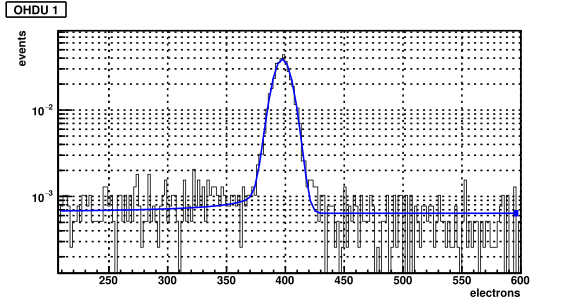
\includegraphics[scale=1]{pngs/OHDU1_EPIX15_sin_correcciones.png}
    \caption{\footnotesize{asd.}}
    \label{fig:OHDU1_EPIX15}
\end{figure}
y finalmente, en tercer lugar se aplican las correcciones en el programa y se generan los histogramas con sus ajustes, de los cuales se desprenden los resultados de este trabajo: El factor de Fano resultó $F = 0.1327 \pm 0.0069$ y la energía de creación electrón hueco $\varepsilon_{\eh} = 3.7224 \pm 0.0000$
\begin{figure}[H]
    \centering
        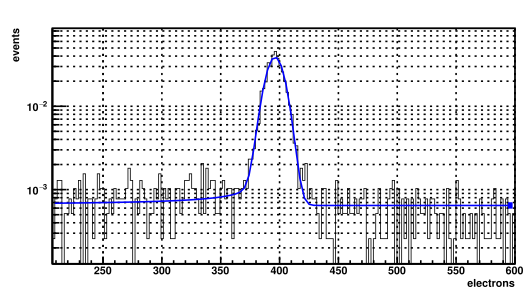
\includegraphics[scale=1]{pngs/OHDU1_EPIX15_Correcciones.png}
    \caption{\footnotesize{asd.}}
    \label{fig:OHDU1_EPIX15_corregido}
\end{figure}
Los resultados para los demás cuadrantes se muestran en las tablas bla y ble
\begin{table}[H]
\centering
\begin{tabular}{@{}ccccc@{}}
\toprule
                & \multicolumn{2}{c}{OHDU1}                 & \multicolumn{2}{c}{OHDU2}                 \\ \midrule
                & $F$                 & $\varepsilon_{\eh}$ & $F$                 & $\varepsilon_{\eh}$ \\
Sin correciones & $0.1322 \pm 0.0022$ & $3.7141 \pm 0.0019$ & $0.1401 \pm 0.0117$ & $3.7149 \pm 0.0037$ \\
EPIX 0.5 (100c) & $0.1322 \pm 0.0022$ & $3.7141 \pm 0.0019$ & $0.1401 \pm 0.0117$ & $3.7149 \pm 0.0037$ \\
EPIX 1.5 y correcciones    & $0.1327 \pm 0.0069$ & $3.7224 \pm 0.0000$ & $0.1399 \pm 0.000$ & $3.7239 \pm 0.0000$ \\ \bottomrule
\end{tabular}
\caption{tabla}
\label{tab:Correciones0}
\end{table}
\begin{table}[H]
\centering
\begin{tabular}{@{}ccccc@{}}
\toprule
                & \multicolumn{2}{c}{OHDU3}                 & \multicolumn{2}{c}{OHDU4}                 \\ \midrule
                & $F$                 & $\varepsilon_{\eh}$ & $F$                 & $\varepsilon_{\eh}$ \\
Sin correciones & $0.1498 \pm 0.0029$ & $3.7209 \pm 0.0029$ & $0.1812 \pm 0.0166$ & $3.7305 \pm 0.0041$ \\
EPIX 0.5 (100c) & $0.1322 \pm 0.0022$ & $3.7141 \pm 0.0019$ & $0.1401 \pm 0.0117$ & $3.7149 \pm 0.0037$ \\
EPIX 1.5 y correcciones    & $0.1327 \pm 0.0069$ & $3.7224 \pm 0.0000$ & $0.1399 \pm 0.000$ & $3.7239 \pm 0.0000$ \\ \bottomrule
\end{tabular}
\caption{tabla}
\label{tab:Correciones0.1}
\end{table}

Sección pendiente porque faltan los resultados. Etiam accumsan non nulla porta lacinia. Curabitur auctor neque ac nulla efficitur fringilla. Phasellus euismod ante id elit faucibus, condimentum condimentum dui viverra. Etiam in nunc semper, hendrerit leo at, bibendum orci. Fusce feugiat at velit ut blandit. Maecenas consectetur condimentum elit, vel venenatis diam pharetra ut. Curabitur vel sapien vitae purus placerat rhoncus nec sit amet dui. Cras vehicula dictum dignissim. Donec placerat mauris in nisl feugiat dictum. Nam dui tortor, rhoncus sed metus at, finibus bibendum libero. Sed nec pharetra lacus, ac pretium mauris. Proin a augue commodo, imperdiet ex vitae, aliquet orci. In condimentum elementum metus in bibendum. Sed tempus augue sit amet tellus posuere posuere. In et suscipit eros, nec interdum nulla. Vestibulum blandit, lorem et viverra dapibus, diam lectus ultricies augue, ut gravida justo quam sed ligula.

\begin{table}[]
\begin{tabular}{@{}ccccc@{}}
\toprule
                & \multicolumn{2}{c}{OHDU1}                 & \multicolumn{2}{c}{OHDU2}                 \\ \hline \hline
                & $F$                 & $\varepsilon_{\eh}$ & $F$                 & $\varepsilon_{\eh}$ \\ \hline
Sin correciones & $0.1469 \pm 0.0123$ & $3.7415 \pm 0.0048$ & $0.1397 \pm 0.0187$ & $3.7549 \pm 0.058$  \\
Con correcciones &
  \multicolumn{1}{c}{$0.1459 \pm 0.0150$} &
  \multicolumn{1}{c}{$3.7532 \pm 0.0044$} &
  \multicolumn{1}{c}{$0.1396 \pm 0.0187$} &
  \multicolumn{1}{c}{$3.7538 \pm 0.0059$} \\ \bottomrule
\end{tabular}
\caption{tabla}
\label{tab:OHDU1OHDU2}
\end{table}

\begin{table}[]
\begin{tabular}{@{}ccccc@{}}
\toprule
                      & \multicolumn{2}{c}{OHDU3}                                           & \multicolumn{2}{c}{OHDU4}                      \\ \hline \hline
\multicolumn{1}{c}{} & \multicolumn{1}{c}{$F$} & \multicolumn{1}{c}{$\varepsilon_{\eh}$} & \multicolumn{1}{c}{$F$} & $\varepsilon_{\eh}$ \\ \hline
\multicolumn{1}{c}{Sin correciones} &
  \multicolumn{1}{c}{$0.1583 \pm 0.0146$} &
  \multicolumn{1}{c}{$3.7466 \pm 0.0042$} &
  \multicolumn{1}{c}{$0.1526 \pm 0.0223$} &
  $3.7638 \pm 0.0063$ \\
\multicolumn{1}{c}{Con correcciones} &
  \multicolumn{1}{c}{$0.1584 \pm 0.0145$} &
  \multicolumn{1}{c}{$3.7531 \pm 0.0042$} &
  \multicolumn{1}{c}{$0.1532 \pm 0.0203$} &
  \multicolumn{1}{c}{$3.7711 \pm 0.0063$} \\ \hline
\end{tabular}
\caption{tabla}
\label{tab:Correcciones2}
\end{table}


% Please add the following required packages to your document preamble:
% \usepackage{booktabs}
\begin{table}[]
\begin{tabular}{@{}ccccc@{}}
\toprule
 &
  \multicolumn{2}{c}{OHDU1} &
  \multicolumn{2}{c}{OHDU2} \\ \midrule
 &
  $F$ &
  \multicolumn{1}{c}{$\varepsilon_{\eh}$} &
  $F$ &
  \multicolumn{1}{c}{$\varepsilon_{\eh}$} \\
Sin correciones &
  $0.1371 \pm 0.0108$ &
  \multicolumn{1}{c}{$3.7156 \pm 0.0033$} &
  $0.1437 \pm 0.0117$ &
  \multicolumn{1}{c}{$3.7164 \pm 0.0037$} \\
Correcciones 50c &
  \multicolumn{1}{c}{$0.1459 \pm 0.0150$} &
  $3.7532 \pm 0.0044$ &
  \multicolumn{1}{c}{$0.1396 \pm 0.0187$} &
  $3.7538 \pm 0.0059$ \\
\multicolumn{1}{c}{Correccion 100c} & \multicolumn{1}{c}{$0.1507 \pm 0.0128$} & $3.7516 \pm 0.0039$ & \multicolumn{1}{c}{$0.1566 \pm 0.0130$} & $3.7388 \pm 0.0040$ \\ \bottomrule
\end{tabular}
\caption{tabla}
\label{tab:Correcciones3}
\end{table}


% Please add the following required packages to your document preamble:
% \usepackage{booktabs}
\begin{table}[]
\begin{tabular}{@{}ccccc@{}}
\toprule
                & \multicolumn{2}{c}{OHDU3}                 & \multicolumn{2}{c}{OHDU4}                 \\ \midrule
                & $F$                 & $\varepsilon_{\eh}$ & $F$                 & $\varepsilon_{\eh}$ \\
Sin correciones & $0.1546 \pm 0.0103$ & $3.7225 \pm 0.0029$ & $0.1876 \pm 0.0169$ & $3.7323 \pm 0.0041$ \\
Correcciones 50c & $0.1584 \pm 0.0145$ & $3.7531 \pm 0.0042$ & $0.1532 \pm 0.0203$ & $3.7711 \pm 0.0063$ \\
Correccion 100c & $0.1762 \pm 0.0154$ & $3.7502 \pm 0.0040$ & $0.2013 \pm 0.0196$ & $3.7654 \pm 0.0047$ \\ \bottomrule
\end{tabular}
\caption{tabla}
\label{tab:Correciones4}
\end{table}
Para este capítulo:

EPIX = 1.5 implica que mato todo lo que está debajo de 1.5, trivialmente. NO como pensaba antes que era 2 y menos de 2. Asi que tengo que ver qué threshold use en python. Chequear y corregir lo que corresponda para tener las correcciones correctamente.

Darío me va a pasar a el root de los datos corridos con epix = 1.5 y con el codigo Fano\_pcc blabla corregido (ultima version) donde tengo que implementar las correcciones.

el modelo de la verosimilitud va a ir en esta sección. y me va a pasar el beta con sus errores con su teoria de fondo pero no necesariamente en este capitulo.

agregar el procesamiento de las imágenes: skipper2root y skextract, cómo se usaron y qué hacen más o menos

